% PROTOKOLL Action Item
\documentclass[
   draft=false
  ,paper=a4
  ,twoside=false
  ,fontsize=11pt
  ,headsepline
  ,DIV11
  ,parskip=full+
]{scrartcl} % copied from Thesis Template from HAW

\usepackage[ngerman,english]{babel}
\usepackage[T1]{fontenc}
\usepackage[utf8]{inputenc}

\usepackage[
    left  =4em
   ,right =4em
   ,top   =5em
   ,bottom=5em
]{geometry}

\usepackage{longtable}
\usepackage[german,refpage]{nomencl}

\usepackage{float}
\usepackage{enumitem}
\usepackage{hyperref} % for a better experience

\hypersetup{
   colorlinks=true % if false - links get colored frames
  ,linkcolor=black % color of tex intern links
  ,urlcolor=blue   % color of url links
}

\usepackage{graphicx}
\usepackage{amsmath}

\usepackage{array}   % for \newcolumntype macro
\newcolumntype{L}{>{$}l<{$}} % math-mode version of "l" column type
\newcolumntype{R}{>{$}r<{$}} % math-mode version of "r" column type
\newcolumntype{C}{>{$}c<{$}} % math-mode version of "c" column type

\usepackage{listings}
\lstset{language=C} 
\usepackage{caption}
\usepackage{colortbl}
\definecolor{tabgrey}{rgb}{0.85,0.85,0.85}
%using minted because of the hashtag in bash

\sloppy
\clubpenalty=10000
\widowpenalty=10000
\displaywidowpenalty=10000

\begin{document}

\selectlanguage{ngerman}
% ----------------------------------------------------------------------------
% ---------------------------------------------------------- HIER WAS MACHEN -
% -------------------------------- Metadaten wie namen und Gruppentreffen etc-
\def\titel{AD Praktikum: Aufgabe 09, Graph and Dykstra}


\def\teilnehmer{ 
	& Sönke Peters & \\
    & Karl-Fabian Witte   & \\
}
% -------------------------------------------------- HIER AUFHÖREN ----------




% ------------------------------------------ einige strukturell Definitionen
\newlength{\txtw} %definiere neue länge
\setlength{\txtw}{\textwidth} %setze neue länge auf textbreite
\addtolength{\txtw}{-10\tabcolsep} %subtrahiere -8\cdot textbreite von asdf

\def\me{\myName \newline \footnotesize{\url{\myEmail} } }

% ------------------------------------------------------------------ Inhalt	
\section*{\titel}
\begin{tabular}{l p{0.4\txtw} p{0.4\txtw} }
	\teilnehmer
	& & \\
	& \today & \\
\end{tabular}


\centering
\textbf{Abstract} \\
Die Datenstruktur eines gewichteter Graphen wird auf Adjazenzmatrix und -liste implementiert und der Algorithmus von Dykstra wird auf diesen mit 
einer Komplexitätsuntersuchung ausgewertet. 
\normalsize \flushleft
\section{Aufgabenstellung}
Es sollen zwei Implementationen von dem abstrakten Datentyp Graph 
realisiert werden. Die Komplexität des Dykstras Algorithmus 
ist auf beiden Graphenimplementationen zu messen. Die für den 
Algorithmus wichtigen zusatzinformationen sind nicht im Graphen
selbst gespeichert. 
Zudem sollen zufallsgeneriertere Graphen erstellt werden, welche 
für die Messung der Komplexität verwedet werden.

\subsection{Grapheninterface und Implementationsarten}

\subsubsection{Adjazenzmatrix}

\subsubsection{Adjazenzliste}

\subsection{Graphengenerator}

\subsection{Algorithmus von Dykstra}

\subsection{Zählerintegration}

\section{Messung}

\begin{figure}[htp]
  	\centering
    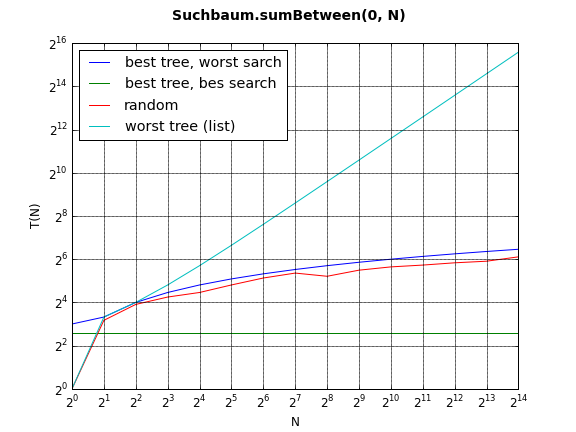
\includegraphics[width=\textwidth]{./IMG/plot.png}
    \caption[shortone]{Aufwende der Suche in Abhängigkeit
     von der Baumstruktur und der geuschten
      Min und Max Werte, sowie der Anzahl der Knoten N}
    \label{fig:plot}
\end{figure}

In Abbildung \ref{fig:plot} zu sehen...


  \begin{lstlisting}
Knoten find_min(int m){
	Knoten a_m = 0;
	Knoten tmp = root;
	Knoten last_gt = root;
	while (a_m == 0){
	  if(m == tmp.wert){
	    a_m = tmp;
	  } else {
	    if ( m < tmp.wert ){
	      last_gt = tmp;
	      if (tmp.linkesKind  == 0) am = last_gt;
	      else                      tmp = tmp.linkesKind;
	    }
	    else if (m > tmp.wert ){
	      if (tmp.rechtesKind  == 0) am = last_gt;
	      else                       tmp = tmp.rechtesKind;
	    }
	}
	return a_m;
}
\end{lstlisting}

\end{document}
% vim: set spell spelllang=de :EOF
